\documentclass[14pt]{extarticle}
\usepackage{lmodern}
\usepackage{amssymb,amsmath}
\usepackage{ifxetex,ifluatex}
\usepackage{fixltx2e} % provides \textsubscript
\ifnum 0\ifxetex 1\fi\ifluatex 1\fi=0 % if pdftex
  \usepackage[T1]{fontenc}
  \usepackage[utf8]{inputenc}
\else % if luatex or xelatex
  \ifxetex
    \usepackage{mathspec}
  \else
    \usepackage{fontspec}
  \fi
  \defaultfontfeatures{Ligatures=TeX,Scale=MatchLowercase}
\fi
% use upquote if available, for straight quotes in verbatim environments
\IfFileExists{upquote.sty}{\usepackage{upquote}}{}
% use microtype if available
\IfFileExists{microtype.sty}{%
\usepackage{microtype}
\UseMicrotypeSet[protrusion]{basicmath} % disable protrusion for tt fonts
}{}
\usepackage[margin=0.6in]{geometry}
\usepackage{hyperref}
\hypersetup{unicode=true,
            pdftitle={Linear Regression: Conditions for Inference, Residual Diagnostics},
            pdfborder={0 0 0},
            breaklinks=true}
\urlstyle{same}  % don't use monospace font for urls
\usepackage{color}
\usepackage{fancyvrb}
\newcommand{\VerbBar}{|}
\newcommand{\VERB}{\Verb[commandchars=\\\{\}]}
\DefineVerbatimEnvironment{Highlighting}{Verbatim}{commandchars=\\\{\}}
% Add ',fontsize=\small' for more characters per line
\usepackage{framed}
\definecolor{shadecolor}{RGB}{248,248,248}
\newenvironment{Shaded}{\begin{snugshade}}{\end{snugshade}}
\newcommand{\KeywordTok}[1]{\textcolor[rgb]{0.13,0.29,0.53}{\textbf{#1}}}
\newcommand{\DataTypeTok}[1]{\textcolor[rgb]{0.13,0.29,0.53}{#1}}
\newcommand{\DecValTok}[1]{\textcolor[rgb]{0.00,0.00,0.81}{#1}}
\newcommand{\BaseNTok}[1]{\textcolor[rgb]{0.00,0.00,0.81}{#1}}
\newcommand{\FloatTok}[1]{\textcolor[rgb]{0.00,0.00,0.81}{#1}}
\newcommand{\ConstantTok}[1]{\textcolor[rgb]{0.00,0.00,0.00}{#1}}
\newcommand{\CharTok}[1]{\textcolor[rgb]{0.31,0.60,0.02}{#1}}
\newcommand{\SpecialCharTok}[1]{\textcolor[rgb]{0.00,0.00,0.00}{#1}}
\newcommand{\StringTok}[1]{\textcolor[rgb]{0.31,0.60,0.02}{#1}}
\newcommand{\VerbatimStringTok}[1]{\textcolor[rgb]{0.31,0.60,0.02}{#1}}
\newcommand{\SpecialStringTok}[1]{\textcolor[rgb]{0.31,0.60,0.02}{#1}}
\newcommand{\ImportTok}[1]{#1}
\newcommand{\CommentTok}[1]{\textcolor[rgb]{0.56,0.35,0.01}{\textit{#1}}}
\newcommand{\DocumentationTok}[1]{\textcolor[rgb]{0.56,0.35,0.01}{\textbf{\textit{#1}}}}
\newcommand{\AnnotationTok}[1]{\textcolor[rgb]{0.56,0.35,0.01}{\textbf{\textit{#1}}}}
\newcommand{\CommentVarTok}[1]{\textcolor[rgb]{0.56,0.35,0.01}{\textbf{\textit{#1}}}}
\newcommand{\OtherTok}[1]{\textcolor[rgb]{0.56,0.35,0.01}{#1}}
\newcommand{\FunctionTok}[1]{\textcolor[rgb]{0.00,0.00,0.00}{#1}}
\newcommand{\VariableTok}[1]{\textcolor[rgb]{0.00,0.00,0.00}{#1}}
\newcommand{\ControlFlowTok}[1]{\textcolor[rgb]{0.13,0.29,0.53}{\textbf{#1}}}
\newcommand{\OperatorTok}[1]{\textcolor[rgb]{0.81,0.36,0.00}{\textbf{#1}}}
\newcommand{\BuiltInTok}[1]{#1}
\newcommand{\ExtensionTok}[1]{#1}
\newcommand{\PreprocessorTok}[1]{\textcolor[rgb]{0.56,0.35,0.01}{\textit{#1}}}
\newcommand{\AttributeTok}[1]{\textcolor[rgb]{0.77,0.63,0.00}{#1}}
\newcommand{\RegionMarkerTok}[1]{#1}
\newcommand{\InformationTok}[1]{\textcolor[rgb]{0.56,0.35,0.01}{\textbf{\textit{#1}}}}
\newcommand{\WarningTok}[1]{\textcolor[rgb]{0.56,0.35,0.01}{\textbf{\textit{#1}}}}
\newcommand{\AlertTok}[1]{\textcolor[rgb]{0.94,0.16,0.16}{#1}}
\newcommand{\ErrorTok}[1]{\textcolor[rgb]{0.64,0.00,0.00}{\textbf{#1}}}
\newcommand{\NormalTok}[1]{#1}
\usepackage{graphicx,grffile}
\makeatletter
\def\maxwidth{\ifdim\Gin@nat@width>\linewidth\linewidth\else\Gin@nat@width\fi}
\def\maxheight{\ifdim\Gin@nat@height>\textheight\textheight\else\Gin@nat@height\fi}
\makeatother
% Scale images if necessary, so that they will not overflow the page
% margins by default, and it is still possible to overwrite the defaults
% using explicit options in \includegraphics[width, height, ...]{}
\setkeys{Gin}{width=\maxwidth,height=\maxheight,keepaspectratio}
\IfFileExists{parskip.sty}{%
\usepackage{parskip}
}{% else
\setlength{\parindent}{0pt}
\setlength{\parskip}{6pt plus 2pt minus 1pt}
}
\setlength{\emergencystretch}{3em}  % prevent overfull lines
\providecommand{\tightlist}{%
  \setlength{\itemsep}{0pt}\setlength{\parskip}{0pt}}
\setcounter{secnumdepth}{0}
% Redefines (sub)paragraphs to behave more like sections
\ifx\paragraph\undefined\else
\let\oldparagraph\paragraph
\renewcommand{\paragraph}[1]{\oldparagraph{#1}\mbox{}}
\fi
\ifx\subparagraph\undefined\else
\let\oldsubparagraph\subparagraph
\renewcommand{\subparagraph}[1]{\oldsubparagraph{#1}\mbox{}}
\fi

%%% Use protect on footnotes to avoid problems with footnotes in titles
\let\rmarkdownfootnote\footnote%
\def\footnote{\protect\rmarkdownfootnote}

%%% Change title format to be more compact
\usepackage{titling}

% Create subtitle command for use in maketitle
\newcommand{\subtitle}[1]{
  \posttitle{
    \begin{center}\large#1\end{center}
    }
}

\setlength{\droptitle}{-2em}

  \title{Linear Regression: Conditions for Inference, Residual Diagnostics}
    \pretitle{\vspace{\droptitle}\centering\huge}
  \posttitle{\par}
    \author{}
    \preauthor{}\postauthor{}
    \date{}
    \predate{}\postdate{}
  
\usepackage{soul}
\usepackage{booktabs}

\begin{document}
\maketitle

\subsubsection{\texorpdfstring{All 5 Have Essentially the Same Estimated
Intercept, Slope, \(R^2\), and Residual Standard
Deviation!}{All 5 Have Essentially the Same Estimated Intercept, Slope, R\^{}2, and Residual Standard Deviation!}}\label{all-5-have-essentially-the-same-estimated-intercept-slope-r2-and-residual-standard-deviation}

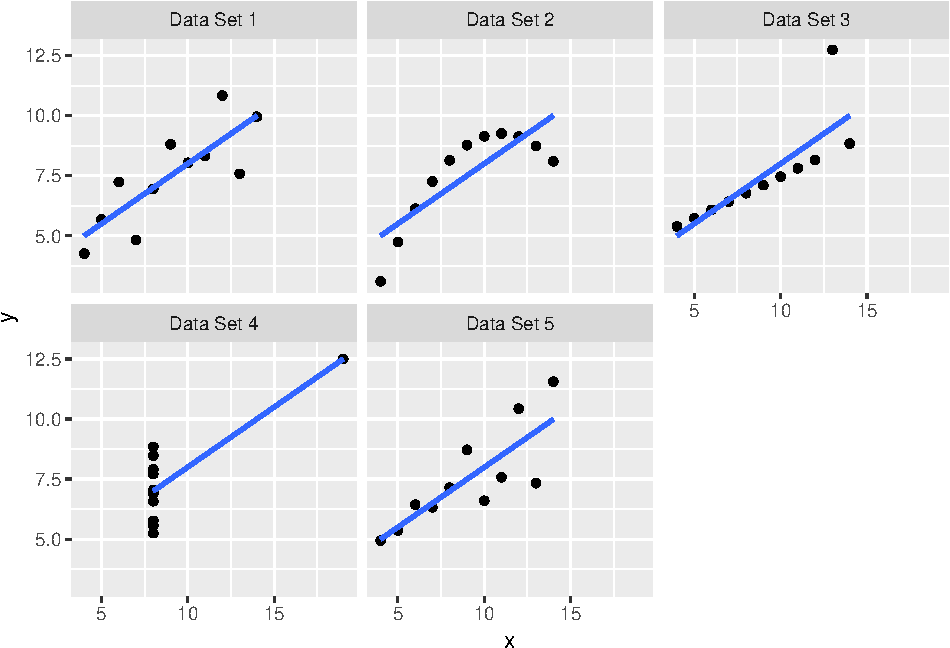
\includegraphics{20181112_anscombe_residuals_files/figure-latex/unnamed-chunk-1-1.pdf}

\begin{itemize}
\tightlist
\item
  Briefly, \textbf{conditions for linear regression} (see last page for
  more detail):

  \begin{itemize}
  \tightlist
  \item
    Sample \textbf{representative} of population
  \item
    No \textbf{outliers} (points that don't fit the trend)
  \item
    \textbf{Linear} relationship
  \item
    \textbf{Independent} observations
  \item
    \textbf{Normally} distributed residuals (or large enough sample
    size)
  \item
    \textbf{Equal variability} of residuals
  \end{itemize}
\item
  \textbf{Use plots} to help diagnose the appropriateness of a linear
  model:

  \begin{itemize}
  \tightlist
  \item
    Scatter plot of explanatory (x axis) vs.~response (y axis)
  \item
    Scatter plot of predicted (x axis) vs.~residual (y axis)
  \item
    Histogram or density plot of residuals (x axis)
  \end{itemize}
\item
  Checks of whether the sample is representative and whether the
  observations are independent come from thinking about data collection
  process, not plots.
\end{itemize}

\newpage

\subsubsection{A Reminder about
Residuals}\label{a-reminder-about-residuals}

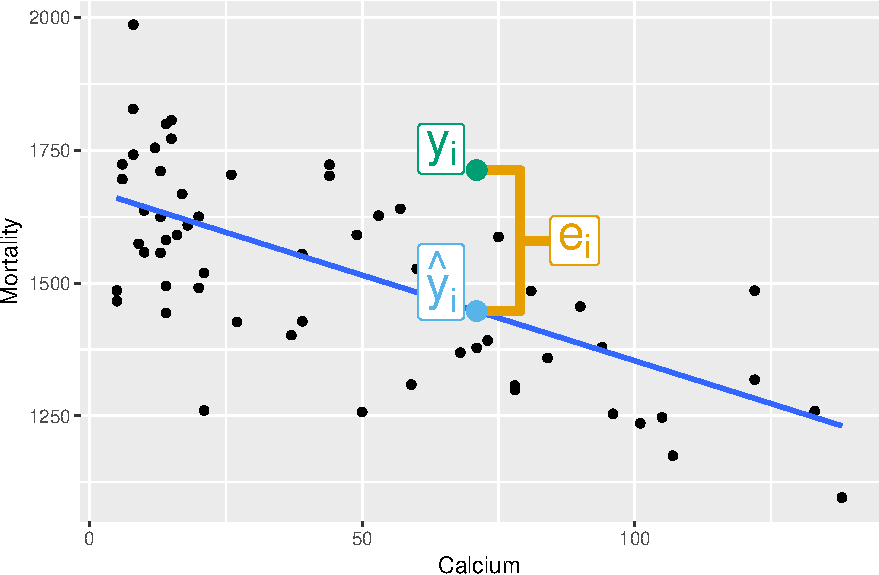
\includegraphics{20181112_anscombe_residuals_files/figure-latex/unnamed-chunk-2-1.pdf}

\begin{itemize}
\item
  Residuals give the vertical distance between a data point and the line
  of best fit
\item
  Positive if point above line, negative otherwise
\item
  \(\definecolor{residual}{RGB}{230,159,0}\color{residual}\text{Residual}\)
  = \(\definecolor{observed}{RGB}{0,158,115}\color{observed}Observed\) -
  \(\definecolor{predicted}{RGB}{86,180,233}\color{predicted}Predicted\)
\item
  \(\definecolor{residual}{RGB}{230,159,0}\color{residual}e_i\) =
  \(\definecolor{observed}{RGB}{0,158,115}\color{observed}y_i\) -
  \(\definecolor{predicted}{RGB}{86,180,233}\color{predicted}\widehat{y}_i\)
  (\(e\) stands for error)
\end{itemize}

\newpage

\subsubsection{Anscombe Quintet: Data Set 1 (All Is
Well)}\label{anscombe-quintet-data-set-1-all-is-well}

\begin{Shaded}
\begin{Highlighting}[]
\KeywordTok{ggplot}\NormalTok{(}\DataTypeTok{data =}\NormalTok{ anscombe, }\DataTypeTok{mapping =} \KeywordTok{aes}\NormalTok{(}\DataTypeTok{x =}\NormalTok{ x1, }\DataTypeTok{y =}\NormalTok{ y1)) }\OperatorTok{+}
\StringTok{  }\KeywordTok{geom_point}\NormalTok{() }\OperatorTok{+}
\StringTok{  }\KeywordTok{geom_smooth}\NormalTok{(}\DataTypeTok{method =} \StringTok{"lm"}\NormalTok{, }\DataTypeTok{se =} \OtherTok{FALSE}\NormalTok{)}
\end{Highlighting}
\end{Shaded}

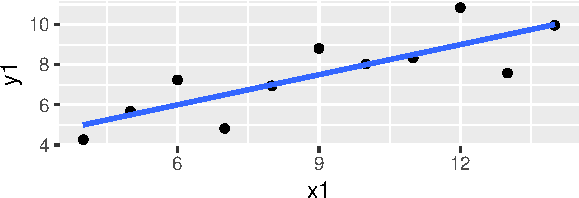
\includegraphics{20181112_anscombe_residuals_files/figure-latex/unnamed-chunk-3-1.pdf}

\begin{Shaded}
\begin{Highlighting}[]
\NormalTok{linear_fit1 <-}\StringTok{ }\KeywordTok{lm}\NormalTok{(y1 }\OperatorTok{~}\StringTok{ }\NormalTok{x1, }\DataTypeTok{data =}\NormalTok{ anscombe)}
\NormalTok{anscombe <-}\StringTok{ }\NormalTok{anscombe }\OperatorTok\StringTok{ }\KeywordTok{mutate}\NormalTok{(}
  \DataTypeTok{predicted1 =} \KeywordTok{predict}\NormalTok{(linear_fit1),}
  \DataTypeTok{residual1 =} \KeywordTok{residuals}\NormalTok{(linear_fit1)}
\NormalTok{)}
\KeywordTok{ggplot}\NormalTok{(}\DataTypeTok{data =}\NormalTok{ anscombe, }\DataTypeTok{mapping =} \KeywordTok{aes}\NormalTok{(}\DataTypeTok{x =}\NormalTok{ predicted1, }\DataTypeTok{y =}\NormalTok{ residual1)) }\OperatorTok{+}
\StringTok{  }\KeywordTok{geom_point}\NormalTok{()}
\end{Highlighting}
\end{Shaded}

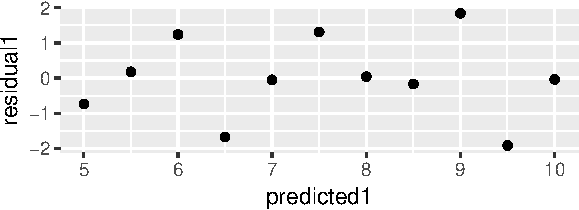
\includegraphics{20181112_anscombe_residuals_files/figure-latex/unnamed-chunk-4-1.pdf}

\begin{Shaded}
\begin{Highlighting}[]
\KeywordTok{ggplot}\NormalTok{(}\DataTypeTok{data =}\NormalTok{ anscombe, }\DataTypeTok{mapping =} \KeywordTok{aes}\NormalTok{(}\DataTypeTok{x =}\NormalTok{ residual1)) }\OperatorTok{+}
\StringTok{  }\KeywordTok{geom_density}\NormalTok{()}
\end{Highlighting}
\end{Shaded}

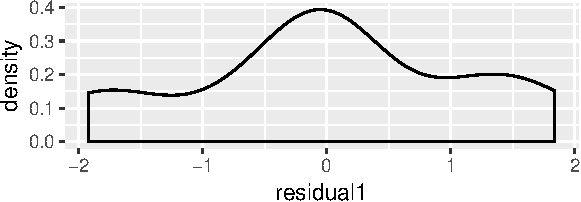
\includegraphics{20181112_anscombe_residuals_files/figure-latex/unnamed-chunk-5-1.pdf}

\begin{itemize}
\item
  \textbf{Outliers}? No
\item
  \textbf{Linear} relationship? Yes
\item
  \textbf{Normally} distributed residuals? Good enough
\item
  \textbf{Equal variability} of residuals? Yes
\end{itemize}

\subsubsection{Anscombe Quintet: Data Set 2
(Nonlinear)}\label{anscombe-quintet-data-set-2-nonlinear}

\begin{Shaded}
\begin{Highlighting}[]
\KeywordTok{ggplot}\NormalTok{(}\DataTypeTok{data =}\NormalTok{ anscombe, }\DataTypeTok{mapping =} \KeywordTok{aes}\NormalTok{(}\DataTypeTok{x =}\NormalTok{ x2, }\DataTypeTok{y =}\NormalTok{ y2)) }\OperatorTok{+}
\StringTok{  }\KeywordTok{geom_point}\NormalTok{() }\OperatorTok{+}
\StringTok{  }\KeywordTok{geom_smooth}\NormalTok{(}\DataTypeTok{method =} \StringTok{"lm"}\NormalTok{, }\DataTypeTok{se =} \OtherTok{FALSE}\NormalTok{)}
\end{Highlighting}
\end{Shaded}

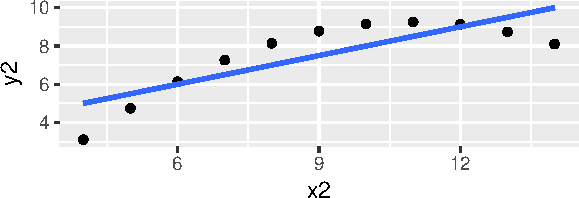
\includegraphics{20181112_anscombe_residuals_files/figure-latex/unnamed-chunk-6-1.pdf}

\begin{Shaded}
\begin{Highlighting}[]
\NormalTok{linear_fit2 <-}\StringTok{ }\KeywordTok{lm}\NormalTok{(y2 }\OperatorTok{~}\StringTok{ }\NormalTok{x2, }\DataTypeTok{data =}\NormalTok{ anscombe)}
\NormalTok{anscombe <-}\StringTok{ }\NormalTok{anscombe }\OperatorTok\StringTok{ }\KeywordTok{mutate}\NormalTok{(}
  \DataTypeTok{predicted2 =} \KeywordTok{predict}\NormalTok{(linear_fit2),}
  \DataTypeTok{residual2 =} \KeywordTok{residuals}\NormalTok{(linear_fit2)}
\NormalTok{)}
\KeywordTok{ggplot}\NormalTok{(}\DataTypeTok{data =}\NormalTok{ anscombe, }\DataTypeTok{mapping =} \KeywordTok{aes}\NormalTok{(}\DataTypeTok{x =}\NormalTok{ predicted2, }\DataTypeTok{y =}\NormalTok{ residual2)) }\OperatorTok{+}
\StringTok{  }\KeywordTok{geom_point}\NormalTok{()}
\end{Highlighting}
\end{Shaded}

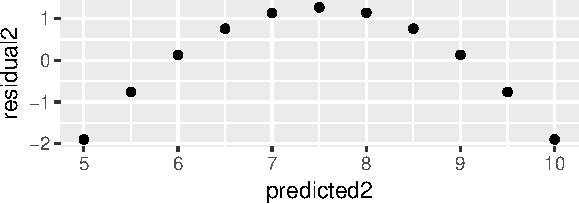
\includegraphics{20181112_anscombe_residuals_files/figure-latex/unnamed-chunk-7-1.pdf}

\begin{Shaded}
\begin{Highlighting}[]
\KeywordTok{ggplot}\NormalTok{(}\DataTypeTok{data =}\NormalTok{ anscombe, }\DataTypeTok{mapping =} \KeywordTok{aes}\NormalTok{(}\DataTypeTok{x =}\NormalTok{ residual2)) }\OperatorTok{+}
\StringTok{  }\KeywordTok{geom_density}\NormalTok{()}
\end{Highlighting}
\end{Shaded}

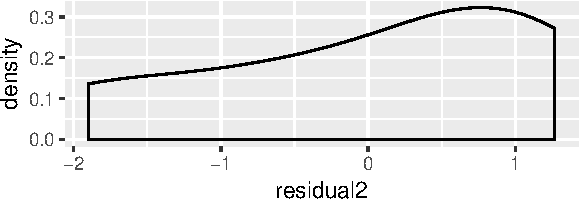
\includegraphics{20181112_anscombe_residuals_files/figure-latex/unnamed-chunk-8-1.pdf}

\begin{itemize}
\item
  \textbf{Outliers}? No
\item
  \textbf{Linear} relationship? No (\textbf{this is a problem!!})
\item
  \textbf{Normally} distributed residuals? No perfect, probably good
  enough
\item
  \textbf{Equal variability} of residuals? Yes
\end{itemize}

\subsubsection{Anscombe Quintet: Data Set 3
(Outlier)}\label{anscombe-quintet-data-set-3-outlier}

\begin{Shaded}
\begin{Highlighting}[]
\KeywordTok{ggplot}\NormalTok{(}\DataTypeTok{data =}\NormalTok{ anscombe, }\DataTypeTok{mapping =} \KeywordTok{aes}\NormalTok{(}\DataTypeTok{x =}\NormalTok{ x3, }\DataTypeTok{y =}\NormalTok{ y3)) }\OperatorTok{+}
\StringTok{  }\KeywordTok{geom_point}\NormalTok{() }\OperatorTok{+}
\StringTok{  }\KeywordTok{geom_smooth}\NormalTok{(}\DataTypeTok{method =} \StringTok{"lm"}\NormalTok{, }\DataTypeTok{se =} \OtherTok{FALSE}\NormalTok{)}
\end{Highlighting}
\end{Shaded}

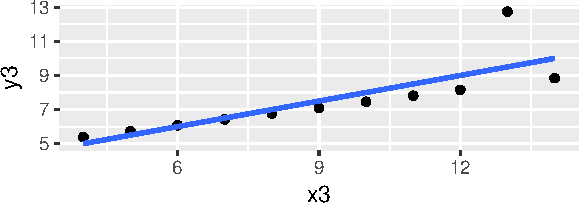
\includegraphics{20181112_anscombe_residuals_files/figure-latex/unnamed-chunk-9-1.pdf}

\begin{Shaded}
\begin{Highlighting}[]
\NormalTok{linear_fit3 <-}\StringTok{ }\KeywordTok{lm}\NormalTok{(y3 }\OperatorTok{~}\StringTok{ }\NormalTok{x3, }\DataTypeTok{data =}\NormalTok{ anscombe)}
\NormalTok{anscombe <-}\StringTok{ }\NormalTok{anscombe }\OperatorTok\StringTok{ }\KeywordTok{mutate}\NormalTok{(}
  \DataTypeTok{predicted3 =} \KeywordTok{predict}\NormalTok{(linear_fit3),}
  \DataTypeTok{residual3 =} \KeywordTok{residuals}\NormalTok{(linear_fit3)}
\NormalTok{)}
\KeywordTok{ggplot}\NormalTok{(}\DataTypeTok{data =}\NormalTok{ anscombe, }\DataTypeTok{mapping =} \KeywordTok{aes}\NormalTok{(}\DataTypeTok{x =}\NormalTok{ predicted3, }\DataTypeTok{y =}\NormalTok{ residual3)) }\OperatorTok{+}
\StringTok{  }\KeywordTok{geom_point}\NormalTok{()}
\end{Highlighting}
\end{Shaded}

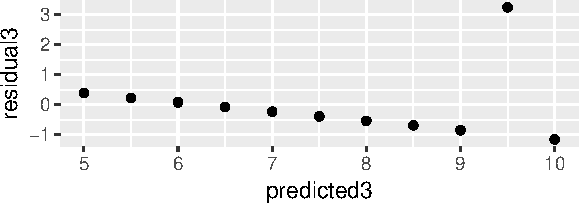
\includegraphics{20181112_anscombe_residuals_files/figure-latex/unnamed-chunk-10-1.pdf}

\begin{Shaded}
\begin{Highlighting}[]
\KeywordTok{ggplot}\NormalTok{(}\DataTypeTok{data =}\NormalTok{ anscombe, }\DataTypeTok{mapping =} \KeywordTok{aes}\NormalTok{(}\DataTypeTok{x =}\NormalTok{ residual3)) }\OperatorTok{+}
\StringTok{  }\KeywordTok{geom_density}\NormalTok{()}
\end{Highlighting}
\end{Shaded}

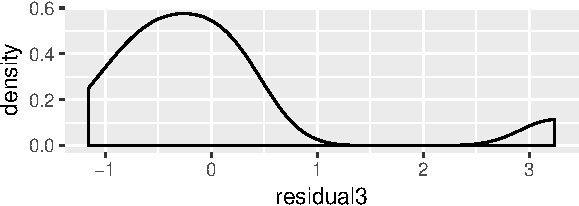
\includegraphics{20181112_anscombe_residuals_files/figure-latex/unnamed-chunk-11-1.pdf}

\begin{itemize}
\item
  \textbf{Outliers}? Yes (\textbf{this is a problem!!})
\item
  \textbf{Linear} relationship? Yes (other than the outlier)
\item
  \textbf{Normally} distributed residuals? No, there is an outlier
\item
  \textbf{Equal variability} of residuals? Yes (other than the outlier)
\end{itemize}

\newpage

\subsubsection{Anscombe Quintet: Data Set 4
(Outlier)}\label{anscombe-quintet-data-set-4-outlier}

\begin{Shaded}
\begin{Highlighting}[]
\KeywordTok{ggplot}\NormalTok{(}\DataTypeTok{data =}\NormalTok{ anscombe, }\DataTypeTok{mapping =} \KeywordTok{aes}\NormalTok{(}\DataTypeTok{x =}\NormalTok{ x4, }\DataTypeTok{y =}\NormalTok{ y4)) }\OperatorTok{+}
\StringTok{  }\KeywordTok{geom_point}\NormalTok{() }\OperatorTok{+}
\StringTok{  }\KeywordTok{geom_smooth}\NormalTok{(}\DataTypeTok{method =} \StringTok{"lm"}\NormalTok{, }\DataTypeTok{se =} \OtherTok{FALSE}\NormalTok{)}
\end{Highlighting}
\end{Shaded}

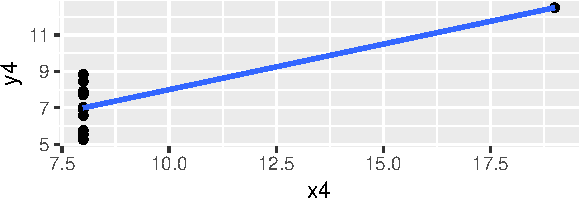
\includegraphics{20181112_anscombe_residuals_files/figure-latex/unnamed-chunk-12-1.pdf}

\begin{Shaded}
\begin{Highlighting}[]
\NormalTok{linear_fit4 <-}\StringTok{ }\KeywordTok{lm}\NormalTok{(y4 }\OperatorTok{~}\StringTok{ }\NormalTok{x4, }\DataTypeTok{data =}\NormalTok{ anscombe)}
\NormalTok{anscombe <-}\StringTok{ }\NormalTok{anscombe }\OperatorTok\StringTok{ }\KeywordTok{mutate}\NormalTok{(}
  \DataTypeTok{predicted4 =} \KeywordTok{predict}\NormalTok{(linear_fit4),}
  \DataTypeTok{residual4 =} \KeywordTok{residuals}\NormalTok{(linear_fit4)}
\NormalTok{)}
\KeywordTok{ggplot}\NormalTok{(}\DataTypeTok{data =}\NormalTok{ anscombe, }\DataTypeTok{mapping =} \KeywordTok{aes}\NormalTok{(}\DataTypeTok{x =}\NormalTok{ predicted4, }\DataTypeTok{y =}\NormalTok{ residual4)) }\OperatorTok{+}
\StringTok{  }\KeywordTok{geom_point}\NormalTok{()}
\end{Highlighting}
\end{Shaded}

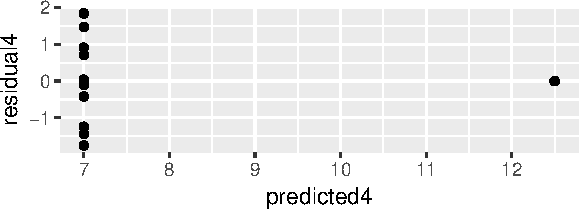
\includegraphics{20181112_anscombe_residuals_files/figure-latex/unnamed-chunk-13-1.pdf}

\begin{Shaded}
\begin{Highlighting}[]
\KeywordTok{ggplot}\NormalTok{(}\DataTypeTok{data =}\NormalTok{ anscombe, }\DataTypeTok{mapping =} \KeywordTok{aes}\NormalTok{(}\DataTypeTok{x =}\NormalTok{ residual4)) }\OperatorTok{+}
\StringTok{  }\KeywordTok{geom_density}\NormalTok{()}
\end{Highlighting}
\end{Shaded}

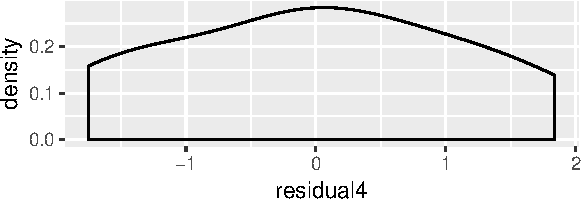
\includegraphics{20181112_anscombe_residuals_files/figure-latex/unnamed-chunk-14-1.pdf}

\begin{itemize}
\item
  \textbf{Outliers}? Yes (\textbf{this is a problem!!})
\item
  \textbf{Linear} relationship? Difficult to assess
\item
  \textbf{Normally} distributed residuals? Yes
\item
  \textbf{Equal variability} of residuals? Difficult to assess
\end{itemize}

\newpage

\subsubsection{Anscombe Quintet: Data Set 5 (Lack of Equal Variability
of
Residuals)}\label{anscombe-quintet-data-set-5-lack-of-equal-variability-of-residuals}

\begin{Shaded}
\begin{Highlighting}[]
\KeywordTok{ggplot}\NormalTok{(}\DataTypeTok{data =}\NormalTok{ anscombe, }\DataTypeTok{mapping =} \KeywordTok{aes}\NormalTok{(}\DataTypeTok{x =}\NormalTok{ x5, }\DataTypeTok{y =}\NormalTok{ y5)) }\OperatorTok{+}
\StringTok{  }\KeywordTok{geom_point}\NormalTok{() }\OperatorTok{+}
\StringTok{  }\KeywordTok{geom_smooth}\NormalTok{(}\DataTypeTok{method =} \StringTok{"lm"}\NormalTok{, }\DataTypeTok{se =} \OtherTok{FALSE}\NormalTok{)}
\end{Highlighting}
\end{Shaded}

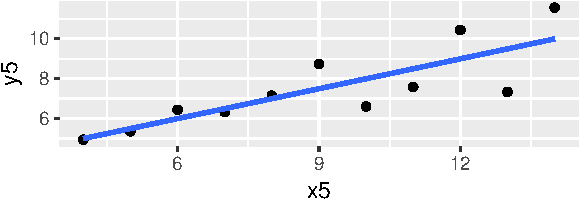
\includegraphics{20181112_anscombe_residuals_files/figure-latex/unnamed-chunk-15-1.pdf}

\begin{Shaded}
\begin{Highlighting}[]
\NormalTok{linear_fit5 <-}\StringTok{ }\KeywordTok{lm}\NormalTok{(y5 }\OperatorTok{~}\StringTok{ }\NormalTok{x5, }\DataTypeTok{data =}\NormalTok{ anscombe)}
\NormalTok{anscombe <-}\StringTok{ }\NormalTok{anscombe }\OperatorTok\StringTok{ }\KeywordTok{mutate}\NormalTok{(}
  \DataTypeTok{predicted5 =} \KeywordTok{predict}\NormalTok{(linear_fit5),}
  \DataTypeTok{residual5 =} \KeywordTok{residuals}\NormalTok{(linear_fit5)}
\NormalTok{)}
\KeywordTok{ggplot}\NormalTok{(}\DataTypeTok{data =}\NormalTok{ anscombe, }\DataTypeTok{mapping =} \KeywordTok{aes}\NormalTok{(}\DataTypeTok{x =}\NormalTok{ predicted5, }\DataTypeTok{y =}\NormalTok{ residual5)) }\OperatorTok{+}
\StringTok{  }\KeywordTok{geom_point}\NormalTok{()}
\end{Highlighting}
\end{Shaded}

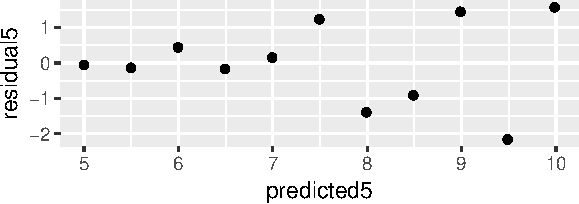
\includegraphics{20181112_anscombe_residuals_files/figure-latex/unnamed-chunk-16-1.pdf}

\begin{Shaded}
\begin{Highlighting}[]
\KeywordTok{ggplot}\NormalTok{(}\DataTypeTok{data =}\NormalTok{ anscombe, }\DataTypeTok{mapping =} \KeywordTok{aes}\NormalTok{(}\DataTypeTok{x =}\NormalTok{ residual5)) }\OperatorTok{+}\StringTok{ }\KeywordTok{geom_density}\NormalTok{()}
\end{Highlighting}
\end{Shaded}

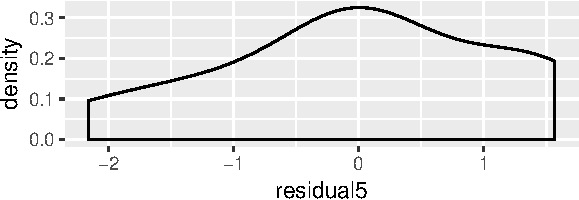
\includegraphics{20181112_anscombe_residuals_files/figure-latex/unnamed-chunk-17-1.pdf}

\begin{itemize}
\item
  \textbf{Outliers}? No
\item
  \textbf{Linear} relationship? Yes
\item
  \textbf{Normally} distributed residuals? Yes
\item
  \textbf{Equal variability} of residuals? No (\textbf{this is a
  problem!!})
\end{itemize}

\newpage

\section{Regression Conditions}\label{regression-conditions}

Think of a helpful leprechaun named \textbf{R}obert \textbf{O'Line}:


\includegraphics[width=0.4\textwidth]{leprechaun.png}

\begin{itemize}
\tightlist
\item
  Sample \textbf{representative} of population
\item
  No \textbf{outliers} (points that don't fit the trend)
\item
  \textbf{Linear} relationship
\item
  \textbf{Independent} observations
\item
  \textbf{Normally} distributed residuals (or large enough sample size)
\item
  \textbf{Equal variability} of residuals
\end{itemize}

\newpage

\begin{table}[htbp]
\centering
\begin{tabular}{p{0.18\textwidth} p{0.2\textwidth} p{0.6\textwidth}}
\toprule
Condition & How Important? & How to Check? \\
\midrule
\textbf{R}epresentative & Critical & Think about data collection (randomization?) \\
\midrule
No \textbf{O}utliers & Very Important & \begin{itemize} \item Scatter Plot of explanatory variable vs response variable \item Scatter plot of predicted value vs residuals \item histogram or density plot of residuals \end{itemize} \\
\midrule
\textbf{L}inear relationship & Very Important & \begin{itemize} \item Scatter Plot of explanatory variable vs response variable (pattern is linear) \item Scatter plot of predicted value vs residuals (no curved patterns) \end{itemize} \\
\midrule
\textbf{I}ndependent observations & Very Important & Think about data collection (randomization?) Situations where observations are \textbf{not} independent: \begin{itemize} \item Observations collected over time (e.g., monthly unemployment measurements over time) \item Multiple observations on the same person (e.g., baseline and follow-up measurements of health in a clinical trial) \end{itemize} \\
\midrule
\textbf{N}ormally distributed residuals & Somewhat Important & \begin{itemize} \item histogram or density plot of residuals (unimodal, approximately symmetric, no outliers)
\item ...or large enough sample size \end{itemize} \\
\midrule
\textbf{E}qual variability of residuals & Somewhat Important & \begin{itemize} \item Scatter Plot of explanatory variable vs response variable (same amount of vertical spread around line for all values of $x$) \item Scatter plot of predicted value vs residuals (same amount of vertical spread for all values of $x$) \end{itemize} \\
\bottomrule
\end{tabular}
\label{table:mr}
\end{table}


\end{document}
